\documentclass[../../../../main.tex]{subfiles}
\begin{document}

$a$ を正の定数とし，
座標平面上に3点 $P_0(1,0)$，$P_1(0,a)$，$P_2(0,0)$ が与えられたとする．

$P_2$ から $P_0P_1$ に垂線をおろし，それと $P_0P_1$ との交点を $P_3$ とする．

$P_3$ から $P_1P_2$ に垂線をおろし，それと $P_1P_2$ との交点を $P_4$ とする．

以下同様にくり返し，一般に $P_n$ が得られたとき，

$P_n$ から $P_{n-2}P_{n-1}$ に垂線をおろし，
それと $P_{n-2}P_{n-1}$ との交点を $P_{n+1}$ とする．

このとき次の問に答えよ．

\begin{figure}[htbp]
  \centering
  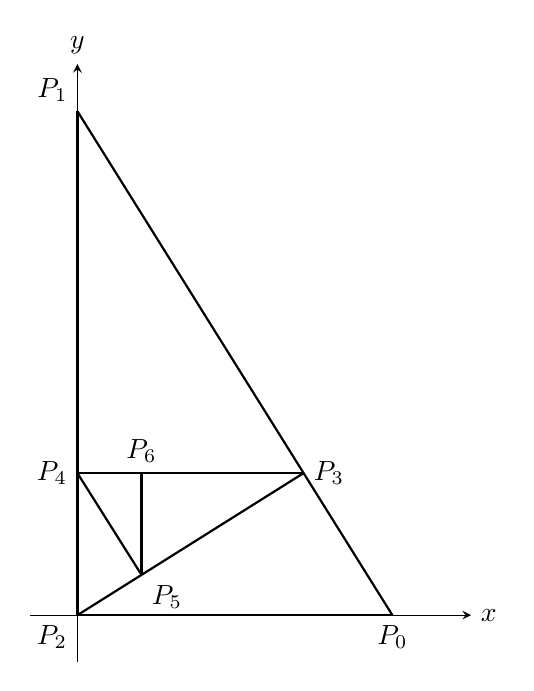
\begin{tikzpicture}[scale=2, >=stealth]
    \draw[->] (-0.3,0) -- (2.5,0) node[right] {$x$};
    \draw[->] (0,-0.3) -- (0,3.5) node[above] {$y$};

    \coordinate (P0) at (2.0, 0);
    \coordinate (P1) at (0, 3.2);
    \coordinate (P2) at (0, 0);

    \coordinate (P3) at (1.436, 0.902);
    \coordinate (P4) at (0, 0.902);
    \coordinate (P5) at (0.407, 0.256);
    \coordinate (P6) at (0.407, 0.902);

    \draw[thick] (P1) -- (P0) node[below] {$P_0$};
    \draw[thick] (P1) -- (P2) node[below left] {$P_2$};
    \draw[thick] (P2) -- (P0);
    \draw[thick] (P2) -- (P3) node[right] {$P_3$};
    \draw[thick] (P3) -- (P4) node[left] {$P_4$};
    \draw[thick] (P4) -- (P5) node[below right] {$P_5$};
    \draw[thick] (P5) -- (P6) node[above] {$P_6$};

    \node[above left] at (P1) {$P_1$};
  \end{tikzpicture}
\end{figure}

\begin{enumerate}
  \item $P_6$ の座標を求めよ．
  \item 上の操作をつづけていくとき，$P_0,P_1,P_2,\cdots,P_n,\cdots$ はどのような点に限りなく近づくか．
\end{enumerate}

\end{document}
